\chapter{Approach}
\label{chap:approach}
This chapter describes the baseline model-based designs and the simulation test approach used to evaluate the data-driven control techniques.

\section{Baseline Designs}
\label{sect:results:baseline}
This section illustrates the baseline performance of the nominal case study systems under static $\mathcal{H}_{2}$ and $\mathcal{H}_{\infty}$ state feedback control.  Both baseline controllers are designed using a fully-known plant, so that the performance of data-driven techniques can be evaluated relative to that which would have been achieved with full model knowledge.

\subsection{Singular Values}
The specific use of singular values in this context is to evaluate the $\mathcal{H}_{\infty}$ norm of the transfer function between disturbances/uncertainty and performance.  In all plots below, the magnitudes of worst-case ``disturbance gain'' is normalized (divided by) the respective minimax/optimal $\gamma^{*}$ as determined via $\mathcal{H}_{\infty}$ optimal control design.  Note that in decibels, this is equivalent to subtracting by $\gamma^{*}$.

One pattern which emerged right away was that the $\mathcal{H}_{\infty}$ controller for $\gamma = \gamma^{*}$ results in a maximum singular value which is totally ``flat'' at $\gamma^{*}$.  While this is indeed optimal by definition, the resulting feedback system is extremely sensitive to variation in the feedback loop, in particular higher-frequency noise.  This phenomenon is not explicitly discussed in the game-theoretic treatment of $\mathcal{H}_{\infty}$ provided by \cite{bacsar2008h}, but it may be understood qualitatively using the ``waterbed effect'' (or by Gunter Stein's ``dirt-shoveling'' analogy \cite{stein2003respect}).  Figure \ref{fig:waterbed_effect} shows the effect of incrementally increasing values of $\gamma$ on the loop shape of the disturbance transfer function.  In particular, the controller begins to attenuate higher frequencies while maintaining a flat (albeit larger-magnitude) response to lower frequencies.

With this observation and some trial-and-error tuning, a fudge factor of 50\% was determined as an acceptable relaxation of the original $\mathcal{H}_{\infty}$ problem.  This means that, for design purposes, $\gamma = 1.5\gamma^{*}$ (or, in decibels, $\gamma_{dB} = \gamma^{*}_{dB}$ + 3.52 dB).  These are shown in the bottom-most row of Figure \ref{fig:waterbed_effect}.  While this design is conservative, the extra attenuation at higher frequencies plays a role in helping to smooth out the effect of unfiltered measurement noise.  Traditional frequency-domain approaches to $\mathcal{H}_{\infty}$ design may have achieved this by lumping frequency-dependent weights into the plant model in order to shape the loop.  However, the fudge factor approach was simplest in the context of this work.

Another observation is that the value of $\gamma$ associated with the $\mathcal{H}_{\infty}$ solution given by MATLAB's \texttt{hinfsyn} routine from its Robust Control Toolbox is slightly higher than the minimax $\gamma^{*}$ produced by bisection.  In Figure \ref{fig:waterbed_effect}, MATLAB's $\mathcal{H}_{\infty}$ solution (the blue curve) is constant and computed separately.  However, when the custom DGARE solver developed for this work (based on policy iteration as described in Appendix \ref{appendix:numerical:iterative}) is initialized with MATLAB's $\gamma^{*}$, it reproduces \texttt{hinfsyn}'s $\mathcal{H}_{\infty}$ solution within numerical precision.  Because no frequency-dependent performance weighting is used, the observed differences in the $\mathcal{H}_{\infty}$ synthesis procedure can be thus be attributed to constraints on the search for $\gamma$.  This highlights a subtle point that practical $\mathcal{H}_{\infty}$ design can be somewhat heuristic.

\begin{figure}[H]
\centering
	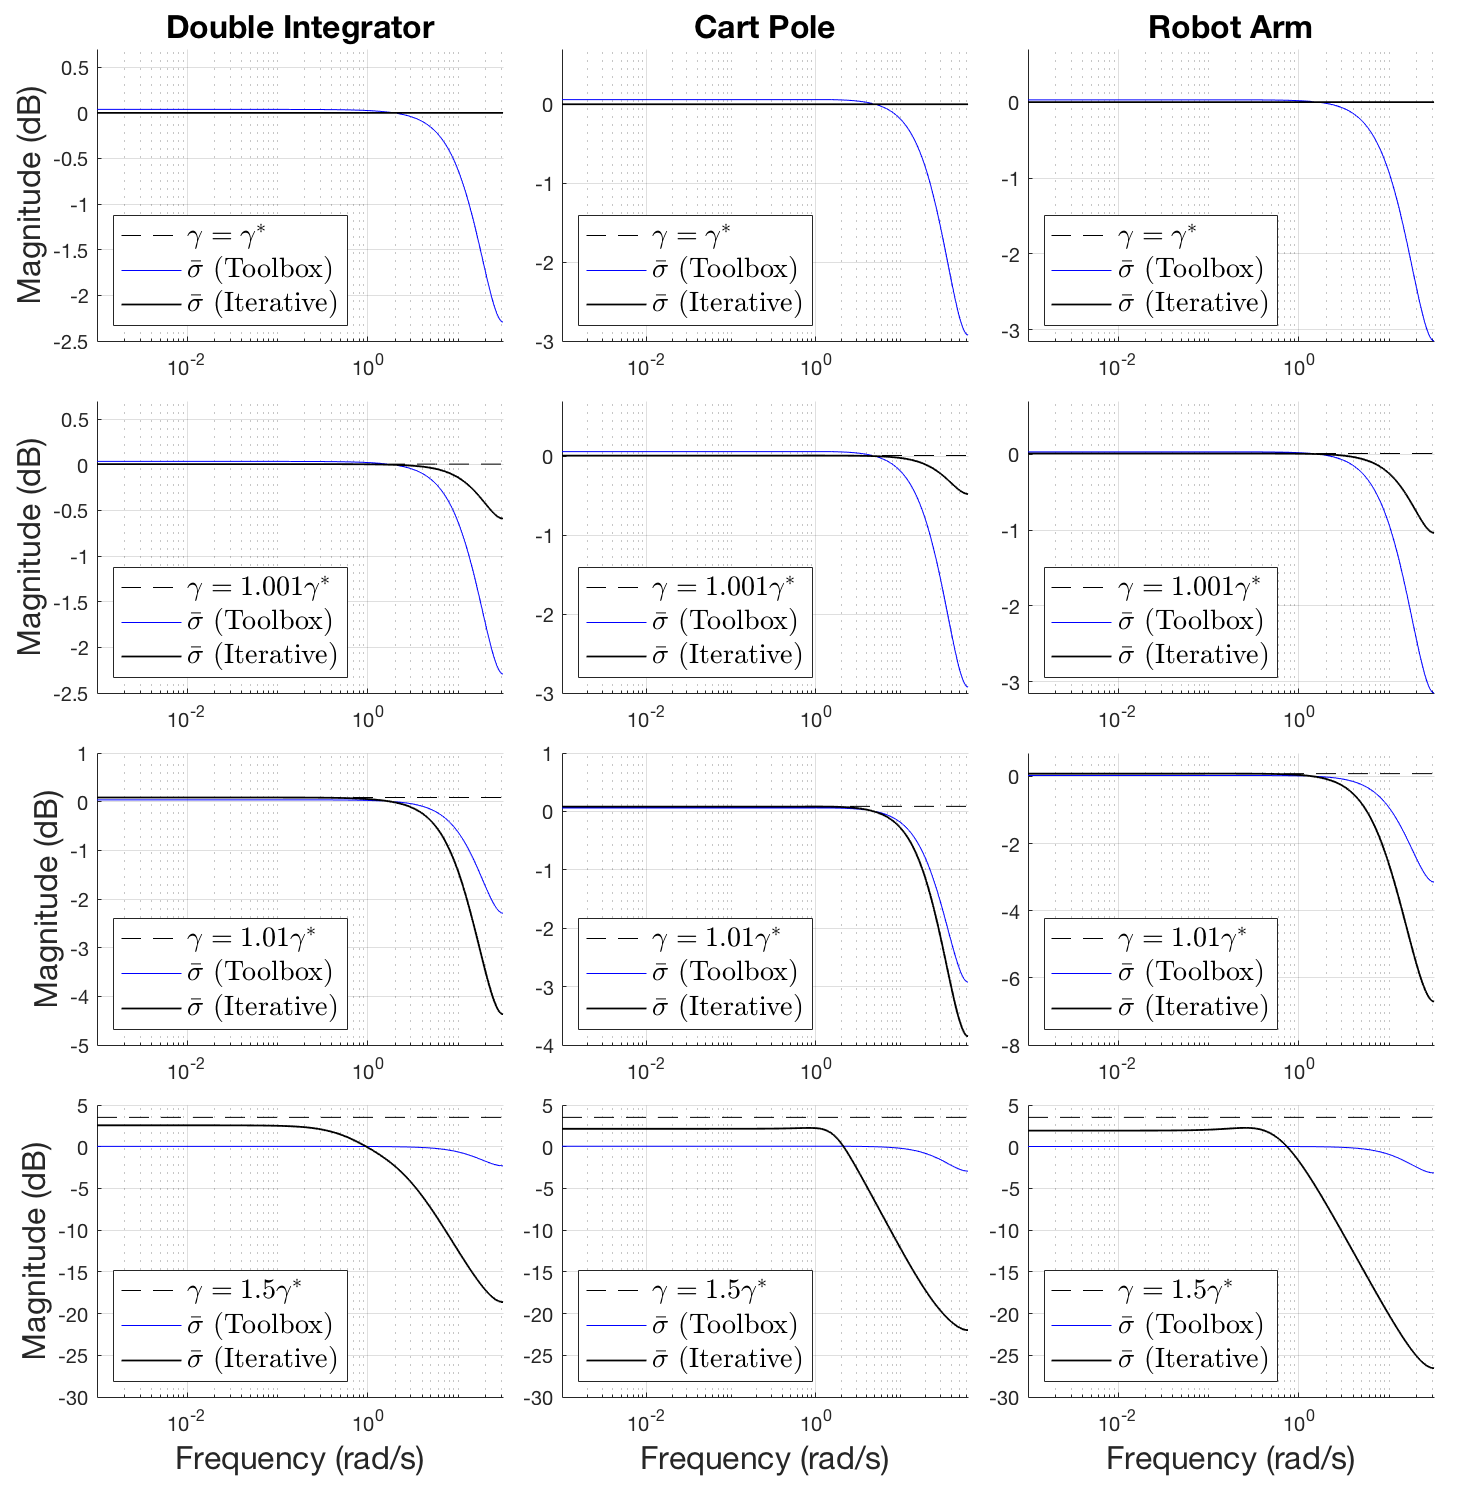
\includegraphics[width=\textwidth]{figures/waterbed_effect.png}
\caption{Loop shape for increasing $\gamma^{*}$, demonstrating the ``waterbed effect''.  Compared are an iterative DGARE solver (black) to \texttt{hinfsyn} from MATLAB's Robust Control Toolbox (blue).}
\label{fig:waterbed_effect}
\end{figure}

Figure \ref{fig:baseline_singular_values} shows the resulting nominal shape of the three case studies' frequency-dependent maximum singular values, relative to their respective minimax/optimal $\gamma^{*}$ (the 0 dB point) and the suboptimal design choice for $\gamma$ used for $\mathcal{H}_{\infty}$ control (the dotted black line).
\begin{figure}[H]
\centering
	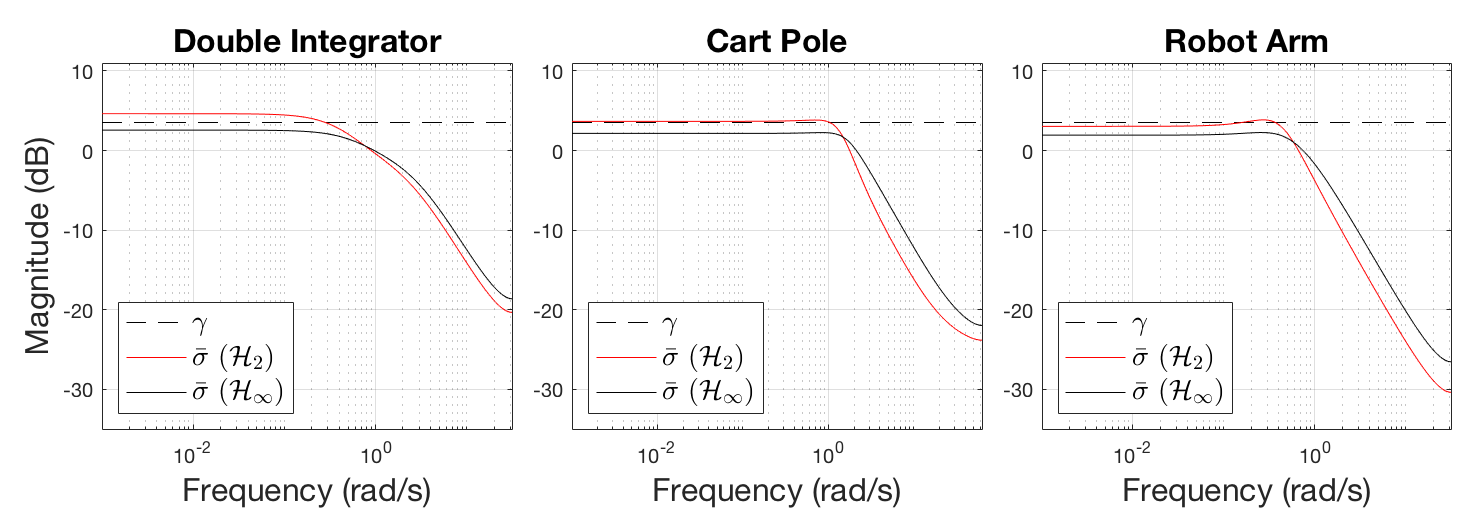
\includegraphics[width=\textwidth]{figures/baseline_singular_values.png}
\caption{Maximum singular values of the closed-loop generalized plants, for baseline controllers.}
\label{fig:baseline_singular_values}
\end{figure}

\subsection{Stability Margins}
One way to express robustness of a feedback system to gain or phase variations is the disk margin \cite{seiler2020introduction}, a scalar quantity which represents how much uncertainty the loop can tolerate before going unstable.  When used for control tuning, disk-based stability margins provide stronger guarantees of robustness than classical gain/phase margins since they take into account the interactions of all loops and frequencies.  In this work, disk-based margins for simultaneous input/output perturbations are computed using MATLAB's \texttt{diskmargin} routine from its Robust Control Toolbox with the known open-loop plant and a given set of feedback gains.  The margins for the baseline systems are listed in Table \ref{table:baseline_disk_margins}.
\begin{table}[H]
\caption{Disk-based stability margins of baseline $\mathcal{H}_{2}$ and $\mathcal{H}_{\infty}$ feedback systems.}
\centering
\begin{tabular}{| l || c | c | c |} 
	\hline
	 & Double Integrator & Cart Pole & Robot Arm\\
	\hline\hline
	Baseline $\mathcal{H}_{2}$ & 1.183 & 0.542 & 0.739\\
	\hline
	Baseline $\mathcal{H}_{\infty}$ & 1.119 & 0.601 & 0.678\\
	\hline
\end{tabular}
\label{table:baseline_disk_margins}
\end{table}

\subsection{Transient Responses}
Figures \ref{fig:baseline_transient_double_integrator}, \ref{fig:baseline_transient_cart_pole} and \ref{fig:baseline_transient_robot_arm} show the transient responses of the three case study systems with the baseline $\mathcal{H}_{2}$ and $\mathcal{H}_{\infty}$ controllers.  The initial conditions of each system are selected to simulate the type of transient response in error dynamics that would immediately follow a closed-loop setpoint command, when the system is already in a stable state (zero velocity or rates).  For the double integrator, this simply means moving the system (e.g. the cart) to another position.  The cart pole moves the system to another position while also stabilizing the pole back to being upright.  The robot arm (without gravity) would similarly be moving from one angular position to another.

\begin{figure}[H]
\centering
	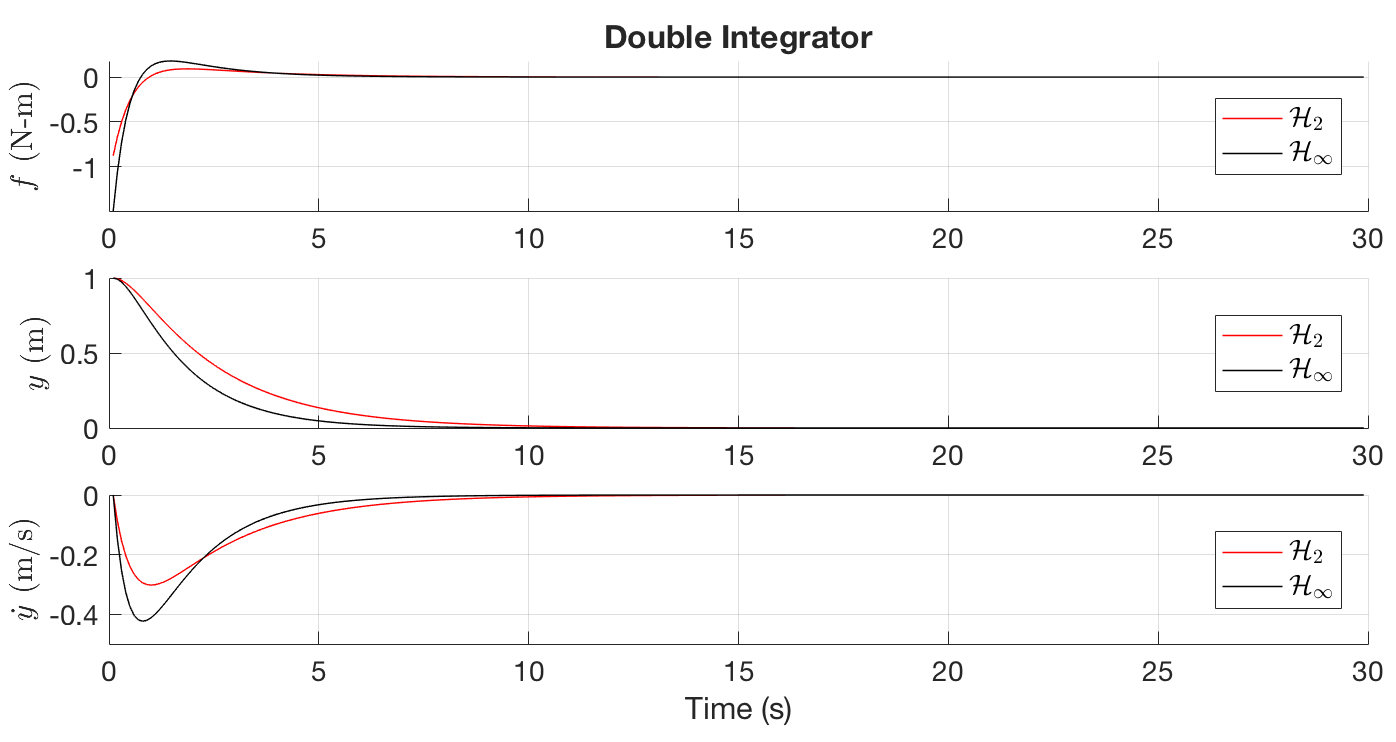
\includegraphics[width=\textwidth]{figures/baseline_transient_double_integrator.png}
\caption{Transient response of the closed-loop double integrator to non-zero initial conditions, for baseline controllers.}
\label{fig:baseline_transient_double_integrator}
\end{figure}

\begin{figure}[H]
\centering
	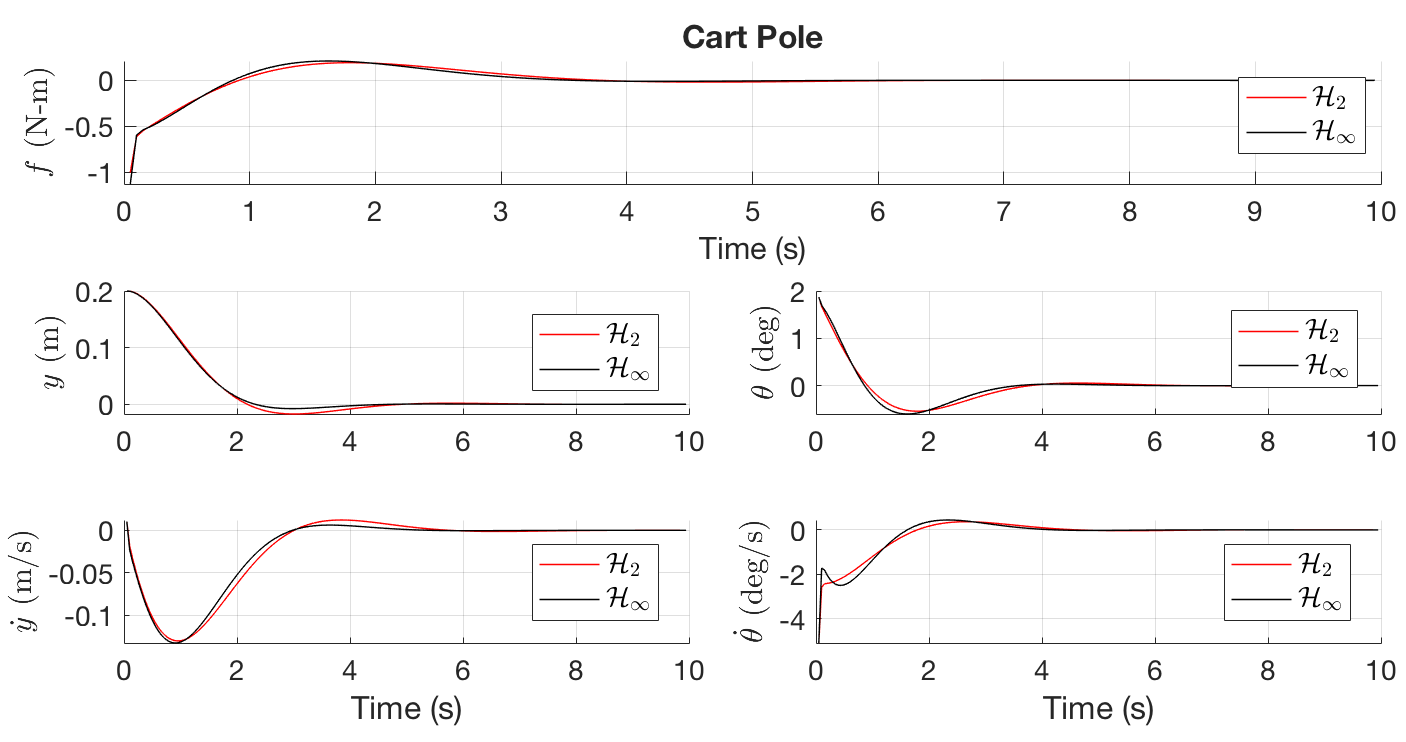
\includegraphics[width=\textwidth]{figures/baseline_transient_cart_pole.png}
\caption{Transient response of the closed-loop cart-pole to non-zero initial conditions, for baseline controllers.}
\label{fig:baseline_transient_cart_pole}
\end{figure}

\begin{figure}[H]
\centering
	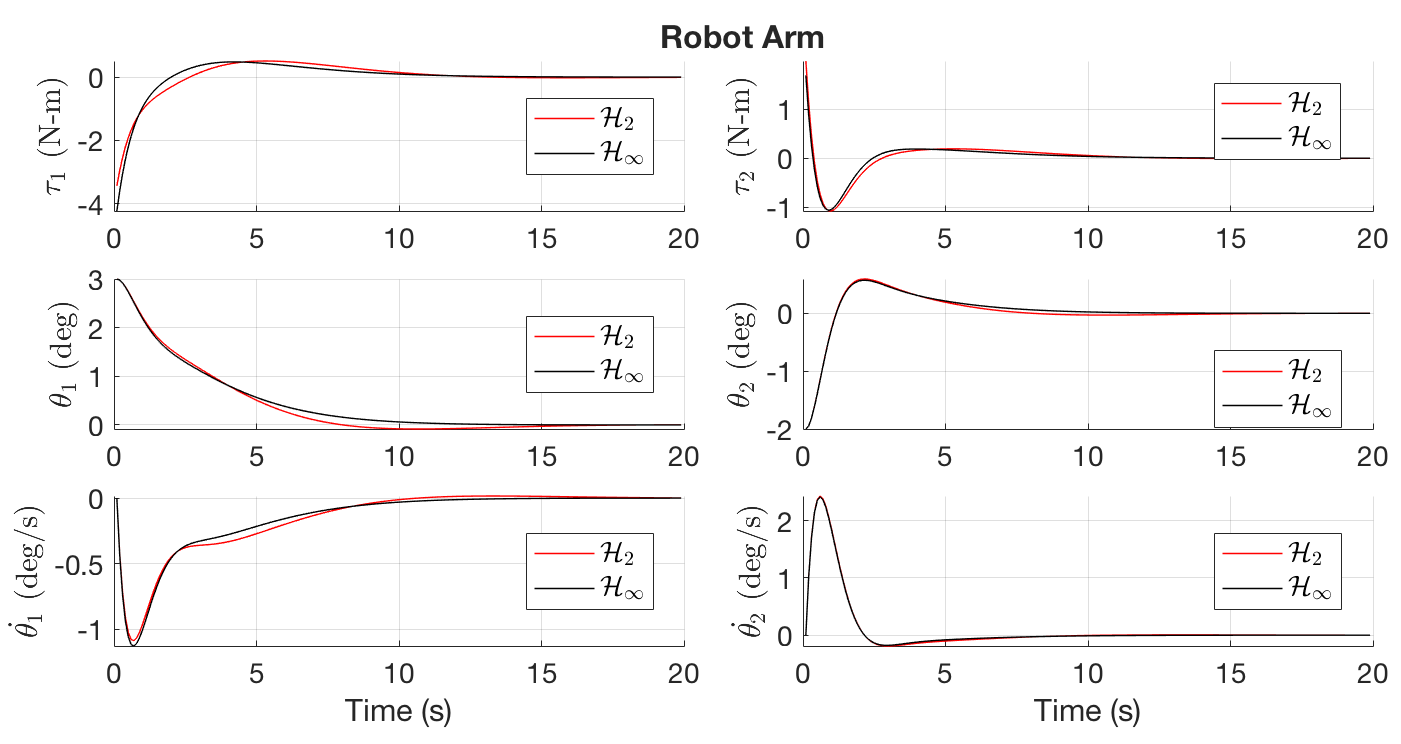
\includegraphics[width=\textwidth]{figures/baseline_transient_robot_arm.png}
\caption{Transient response of the closed-loop robot arm to non-zero initial conditions, for baseline controllers.}
\label{fig:baseline_transient_robot_arm}
\end{figure}

\subsection{Integrated Performance Metrics}
Figures \ref{fig:baseline_integrated_cost} shows the total integrated cost and control effort for each of the three case studies with $\mathcal{H}_{2}$ and $\mathcal{H}_{\infty}$ control.  The $\mathcal{H}_{\infty}$ control requires more control effort in all three cases, which leads to a rise in total LQ cost over the trajectory.  Note that in Figure \ref{fig:baseline_integrated_cost}, the integrated cost and control effort are both normalized to the infinite-horizon LQR cost.  This allows a standard comparison of performance relative to that which would be achieved with perfect model knowledge and zero disturbances.  The LQ cost plotted in the top row of Figure \ref{fig:baseline_integrated_cost} is given by Equation \ref{eq-optimal-cost-function}, and the control effort plotted in the bottom row of Figure \ref{fig:baseline_integrated_cost} is given by Equation \ref{eq:total-integrated-control-effort}.
\begin{equation}
\label{eq:total-integrated-control-effort}
\begin{aligned}
	J_{u} &= \lim_{N \to \infty} \sum_{k = 1}^{N} \big{(} \vb*{u}_{k}^{T} \vb*{u}_{k} \big{)}
\end{aligned}
\end{equation}

\begin{figure}[H]
\centering
	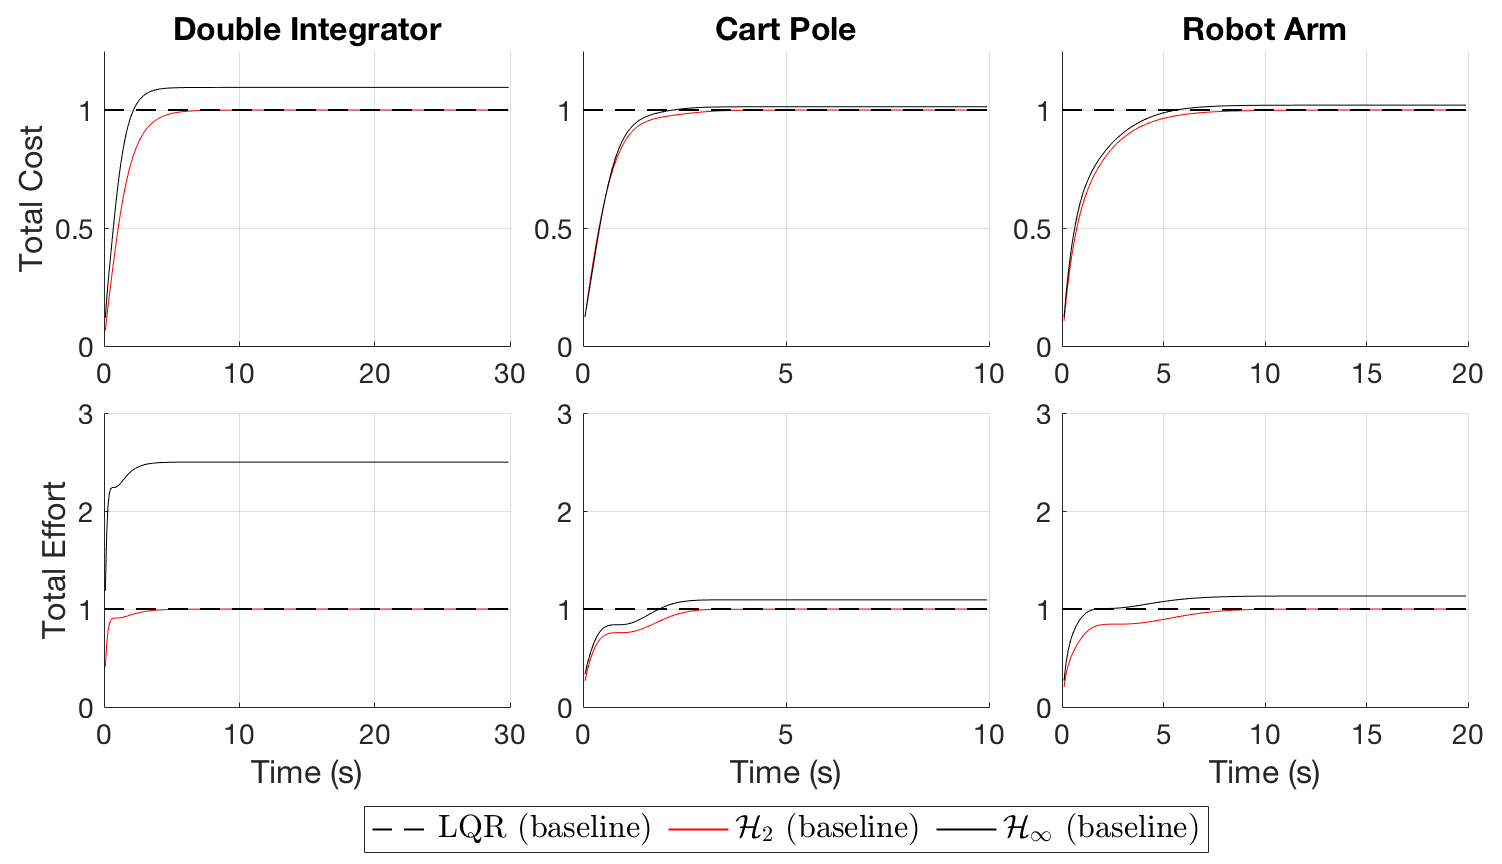
\includegraphics[width=\textwidth]{figures/baseline_integrated_cost.png}
\caption{Integrated cost and control effort of the closed-loop systems to non-zero initial conditions, for baseline controllers.}
\label{fig:baseline_integrated_cost}
\end{figure}

\section{Simulation Test Approach}
\label{sect:results:testapproach}
To test the effect of uncertainty and noise on both indirect and direct data-driven control, a repeated-trial test is used to evaluate each case study.  There are two test scenarios: learning to control a system with parameter uncertainty, and learning to control a system with measurement noise.  It is expected that while measurement noise should have no effect on the ability to compute baseline control designs, it will certainly affect the efficacy of learning controllers from data, and may affect the performance of both types when simulated.

For a separate sweep of each of the two scale factors (from 0\% to 60\%), 100 different test runs are evaluated for different data-driven control methods in order to compare to baseline model-based control methods.  Each run gathers a finite trajectory of training data from the fully-nonlinear plant, and using this data, several data-driven controllers are computed.  If they are stable, their robustness metrics are compared to the baseline case.

Indirect approaches use the DMDc algorithm given by Equation \eqref{eq:dmdc_solution} to estimate a linear discrete-time plant model from the training data, followed by model-based $\mathcal{H}_{2}$ and (suboptimal) $\mathcal{H}_{\infty}$ control.  Direct approaches implement the LMIs given by Equations \eqref{eq:h2_lmi_dd} and \eqref{eq:h2s_lmi_dd} that solve model-free optimizations for $\mathcal{H}_{2}$ optimal and $\mathcal{H}_{2}$ suboptimal control, respectively.  These leverage the MATLAB-based CVX parser \cite{grant2008graph, grant2008cvx} with its default SDPT3 \cite{toh1999sdpt3, tutuncu2001sdpt3} and SeDuMi \cite{sturm1999using} SDP solvers.

For a given scale factor, several metrics are computed and averaged across the 100 test runs.  The first metric is the fraction of stabilizing data-driven controllers; those that do not keep the system poles within the unit circle are marked as unstable.  For those that are stable, the closed-loop disk margin (see Appendix \ref{appendix:sensitivity}) and $\mathcal{H}_{\infty}$ norms are compared to characterize the robustness of the controllers synthesized from data.

Additionally, the full feedback system is then simulated with fixed duration and initial conditions to obtain integrated control effort and LQ cost, to characterize performance.  However, those whose integrated metrics or $\mathcal{H}_{\infty}$ norms are disproportionately large (at least 10 times above the average) are marked unstable and their metrics are discarded.

\underline{\textbf{Note:}} Because unstable controllers cannot be included in the calculation of robustness metrics, average values (nominally out of 100 samples) become skewed when the fraction of stable controllers dwindles

\subsection{Training Policies}
Table \ref{table:training_policies} summarizes the control policies used to gather an $N$-sample state-input trajectory of training data.  In general, these were a linear combination of a stabilizing state feedback law with gains $\vb*{K}_{0}$, a time-varying input $\vb*{u}_{expl}(t_{k})$ to promote exploration, i.e.,
\begin{equation}
\begin{aligned}
	\vb*{u} &= \vb*{K}_{0}\vb*{x}_{k} + \vb*{u}_{expl}(t_{k})
\end{aligned}
\end{equation}
and the values of $\vb*{K}_{0}$ were selected heuristically.   These merely keep the closed-loop system stable, and are generally not optimized for robustness or performance.
\begin{table}[H]
\caption{Control policies used to gather training data.}
\centering
\begin{tabular}{|c || c | c | c|} 
	\hline
	 & $\vb*{K}_{0}$ & $\vb*{u}_{expl}(t_{k})$ & $N$\\
	\hline\hline
	Double Integrator & $\begin{bmatrix} -1.91 & -1.01\end{bmatrix}$ & $0.1\exp(-0.8t_{k})\sin(4t_{k}) + \mathcal{N}(0, 0.5)$ & 80\\ 
	\hline
	Cart Pole & $\begin{bmatrix}-2 & 3 & -3 & 7\end{bmatrix}$ & $10.1\exp(-0.8t_{k})\sin(t_{k})$ & 100\\
	\hline
	Robot Arm & $\begin{bmatrix}-60 & -3 & -200 & -60\\ -3 & -60 & -60 & -68\end{bmatrix}$ & $\begin{bmatrix}
		10\exp(-0.8t_{k})\sin(t_{k}) + \mathcal{N}(0, 0.05)\\ 10\exp(-0.8t_{k})\sin(t_{k}) + \mathcal{N}(0, 0.05) \end{bmatrix}$ & 150\\
	\hline
\end{tabular}
\label{table:training_policies}
\end{table}

\newpage
\subsection{Parameter Uncertainty Test Harness}
Here, a single inertial parameter from each case study system was selected to be uncertain.  For the double integrator, this was the mass ($m_{c}$), for the cart-pole it was the pole length ($l$) and for the robot arm this was the length of link 1 ($l_{1}$).  These parameters were subjected to a zero-mean Gaussian additive disturbance with a variance that is some fraction of their nominal value.  Pseudocode for this test is given by Algorithm \ref{alg:scaled_uncertainty_test}, which is applied to each of the three case studies.

\begin{algorithm}
\caption{Test harness for simulating single parameter uncertainty.}
\label{alg:scaled_uncertainty_test}
\begin{algorithmic}
	\State Calculate baseline model-based control gains ($\mathcal{H}_{2}$, $\mathcal{H}_{\infty}$):
	\State \hspace{10pt} $\vb*{K}_{2}^{b} \gets $ baseline $\mathcal{H}_{2}$ synthesis
	\State \hspace{10pt} $\vb*{K}_{\infty}^{b} \gets $ baseline $\mathcal{H}_{\infty}$ synthesis
	\For{scale factor in $ \begin{bmatrix} 0, & 0.1, & 0.2, & 0.3, & 0.4, & 0.5, & 0.6 \end{bmatrix}$}
		\State $n \gets 1$
		\While{$n < 100$}
			\State Perturb system parameter according to scale factor.
			\State Compute off-nominal linearized plant model.
			\State Simulate full off-nominal system to obtain training data.
			\State Use training data to compute data-driven control gains ($\mathcal{H}_{2}$, $\mathcal{H}_{\infty}$):
			\State \hspace{10pt} $\vb*{K}_{2}^{i} \gets $ indirect $\mathcal{H}_{2}$ synthesis
			\State \hspace{10pt} $\vb*{K}_{2}^{d} \gets $ direct $\mathcal{H}_{2}$ synthesis
			\State \hspace{10pt} $\vb*{K}_{\infty}^{i} \gets $ indirect $\mathcal{H}_{\infty}$ synthesis
			\For{$\tilde{\vb*{K}}$ in $\begin{bmatrix} \vb*{K}_{2}^{b}, & \vb*{K}_{\infty}^{b}, & \vb*{K}_{2}^{i}, & \vb*{K}_{2}^{d}, & \vb*{K}_{\infty}^{i} \end{bmatrix}$}
				\State Use off-nominal plant to compute closed-loop stability of $(\vb*{A} - \vb*{B}\vb*{K})$.
				\If{stable}
					\State Compute disk margin using sensitivity function $(\vb*{S} - \vb*{T})/2$.
					\State Compute $\mathcal{H}_{\infty}$ norm using generalized plant $\vb*{T}_{K}(z)$.
					\State Simulate full system with $\vb*{u}_{k} = -\tilde{\vb*{K}}\vb*{x}_{k}$, from initial conditions $(\vb*{x}_{0},\vb*{u}_{0})$.
					\State Compute total integrated control effort and total integrated LQ cost.
				\Else
					\State Test failed; discard and set all metrics to NaN.
				\EndIf
			\EndFor
		\State $n \gets n + 1$
		\EndWhile
	\EndFor
\end{algorithmic}
\end{algorithm}

\subsection{Measurement Noise Test Harness}
Here, a rough estimate of nominal variance was assumed for each system.  This was then scaled in a similar fashion as the parameter uncertainty.  Nominal variance was taken as 0.1 m$^{2}$ for position, 0.05 m$^{2}$s$^{-2}$ for linear velocity, 0.1deg$^{2}$ for angles and 0.01deg$^{2}$s$^{-2}$ for angular rates.  Maximum values were taken to be twice the nominal values, and the scale factor was applied to the maximum values.  Pseudocode for this test is given by Algorithm \ref{alg:scaled_noise_test}, which is applied to each of the three case studies.

\begin{algorithm}
\caption{Test harness for simulating measurement noise.}
\label{alg:scaled_noise_test}
\begin{algorithmic}
	\State Calculate baseline model-based control gains ($\mathcal{H}_{2}$, $\mathcal{H}_{\infty}$):
	\State \hspace{10pt} $\vb*{K}_{2}^{b} \gets $ baseline $\mathcal{H}_{2}$ synthesis
	\State \hspace{10pt} $\vb*{K}_{\infty}^{b} \gets $ baseline $\mathcal{H}_{\infty}$ synthesis
	\For{scale factor in $ \begin{bmatrix} 0, & 0.1, & 0.2, & 0.3, & 0.4, & 0.5, & 0.6 \end{bmatrix}$}
		\State Adjust variance of measurement noise according to scale factor.
		\State $n \gets 1$
		\While{$n < 100$}
			\State Simulate full noisy system to obtain training data.
			\State Use training data to compute data-driven control gains ($\mathcal{H}_{2}$, $\mathcal{H}_{\infty}$):
			\State \hspace{10pt} $\vb*{K}_{2}^{i} \gets $ indirect $\mathcal{H}_{2}$ synthesis
			\State \hspace{10pt} $\vb*{K}_{2}^{d} \gets $ direct $\mathcal{H}_{2}$ synthesis
			\State \hspace{10pt} $\vb*{K}_{\infty}^{i} \gets $ indirect $\mathcal{H}_{\infty}$ synthesis
			\For{$\tilde{\vb*{K}}$ in $\begin{bmatrix} \vb*{K}_{2}^{b}, & \vb*{K}_{\infty}^{b}, & \vb*{K}_{2}^{i}, & \vb*{K}_{2}^{d}, & \vb*{K}_{\infty}^{i} \end{bmatrix}$}
				\State Use nominal plant to compute closed-loop stability of $(\vb*{A} - \vb*{B}\vb*{K})$.
				\If{stable}
					\State Compute disk margin using sensitivity function $(\vb*{S} - \vb*{T})/2$.
					\State Compute $\mathcal{H}_{\infty}$ norm using generalized plant $\vb*{T}_{K}(z)$.
					\State Simulate full system with $\vb*{u}_{k} = -\tilde{\vb*{K}}\vb*{x}_{k}$, from initial conditions $(\vb*{x}_{0},\vb*{u}_{0})$.
					\State Compute total integrated control effort and total integrated LQ cost.
				\Else
					\State Test failed; discard and set all metrics to NaN.
				\EndIf
			\EndFor
		\State $n \gets n + 1$
		\EndWhile
	\EndFor
\end{algorithmic}
\end{algorithm}
